\documentclass{article}
\usepackage{amsmath}
\usepackage{enumerate}
\usepackage{listings}
\usepackage{moreverb}
\usepackage[margin=1in]{geometry}
\usepackage{graphicx}
\usepackage{dsfont}
\title{STA 360: Lab 11}
\author{Michael Lin}

\begin{document}
\maketitle

\begin{enumerate}
\item Let $w_i$ be the indicator for whether observation is from a weekday or weekend. In particular, $w_i=1$ with probability $p$ if $i$ is weekday, and $w_i=0$ with probability $1-p$. In other words,
$$w_i\sim \text{Be}(p)$$
Henceforth, let $\xi$ denote the p.d.f. Given $p \sim \text{Beta}(5,2)$, the posterior p.d.f. of $p$ is:
\begin{align*}
\xi(p|w_{1:n}) &\propto \xi(w_{1:n}|p)\xi(p) \\
&=\Big(\prod_{i=1}^{n} p^{w_i}(1-p)^{1-w_i} \Big)\frac{\Gamma(7)}{\Gamma(5)\Gamma(2)}p^4(1-p) \\
&\propto p^{\sum w_i}(1-p)^{n-\sum w_i}p^4(1-p) \\
&=p^{(5+\sum w_i)-1}(1-p)^{(n+b-\sum w_i)-1} \\
&\propto \text{Beta}(p | 5+\sum w_i, n+2-\sum w_i)
\end{align*}

Recall the following distributions:
$$y_i | (w_i=1) \sim \text{LN}(\mu_1, \sigma_1^2)$$
$$y_i | (w_i=0) \sim \text{LN}(\mu_2, \sigma_2^2)$$

Thus by Bayes' Rule:
$$\mathds{P}(w_i=1|y_i, p) = \frac{\frac{1}{y_i \sqrt{2\pi\sigma_1^2}}\exp\{-(\log y_i-\mu_1)^2/2\sigma_1^2\}p}{\frac{1}{y_i \sqrt{2\pi\sigma_1^2}}\exp\{-(\log y_i-\mu_1)^2/2\sigma_1^2\}p + \frac{1}{y_i \sqrt{2\pi\sigma_2^2}}\exp\{-(\log y_i-\mu_2)^2/2\sigma_1^2\}(1-p)}$$

Define $\pi_i = \mathds{P}(w_i=1|y_i, p)$. For each iteration of the Gibb's sampler, we would sample:
$$w_i\sim \text{Be}(\pi_i)$$

Then we would sample $\mu_1, \mu_2, \sigma_1^2, \sigma_2^2$ as we did in lab 10.

See below for derivation of full conditionals from lab 10:

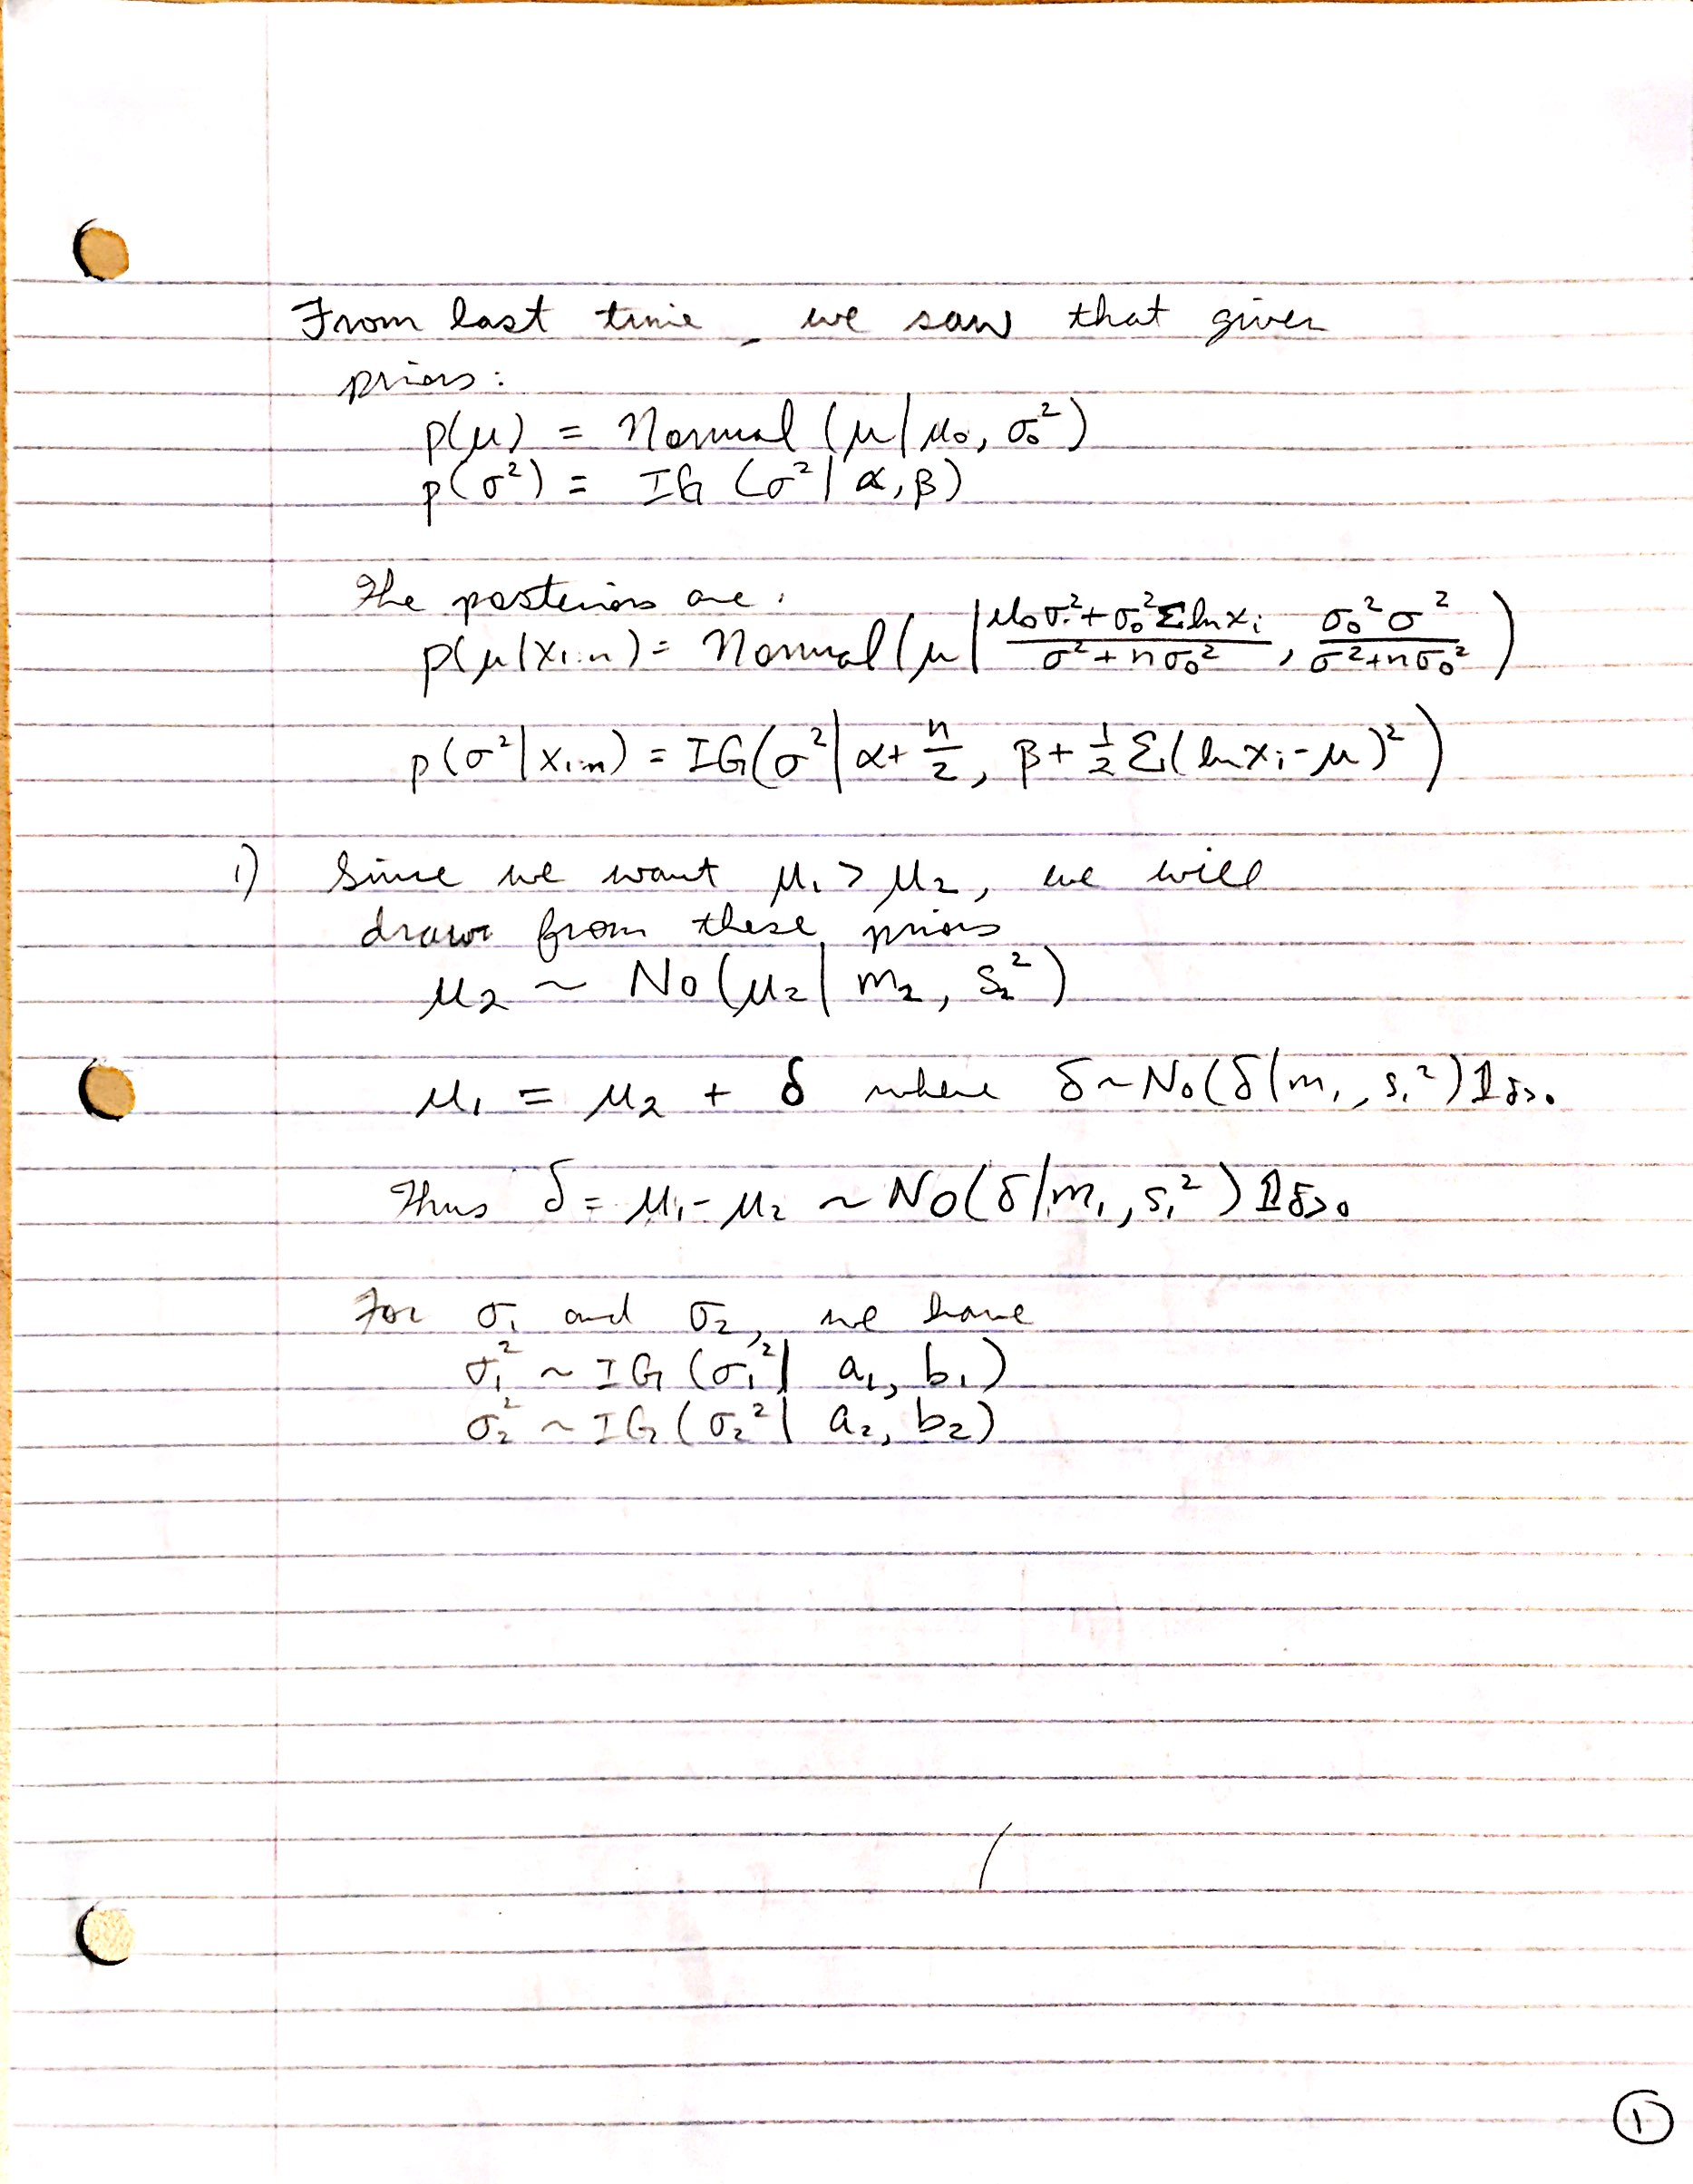
\includegraphics[scale = 0.23]{page1.jpg}\\
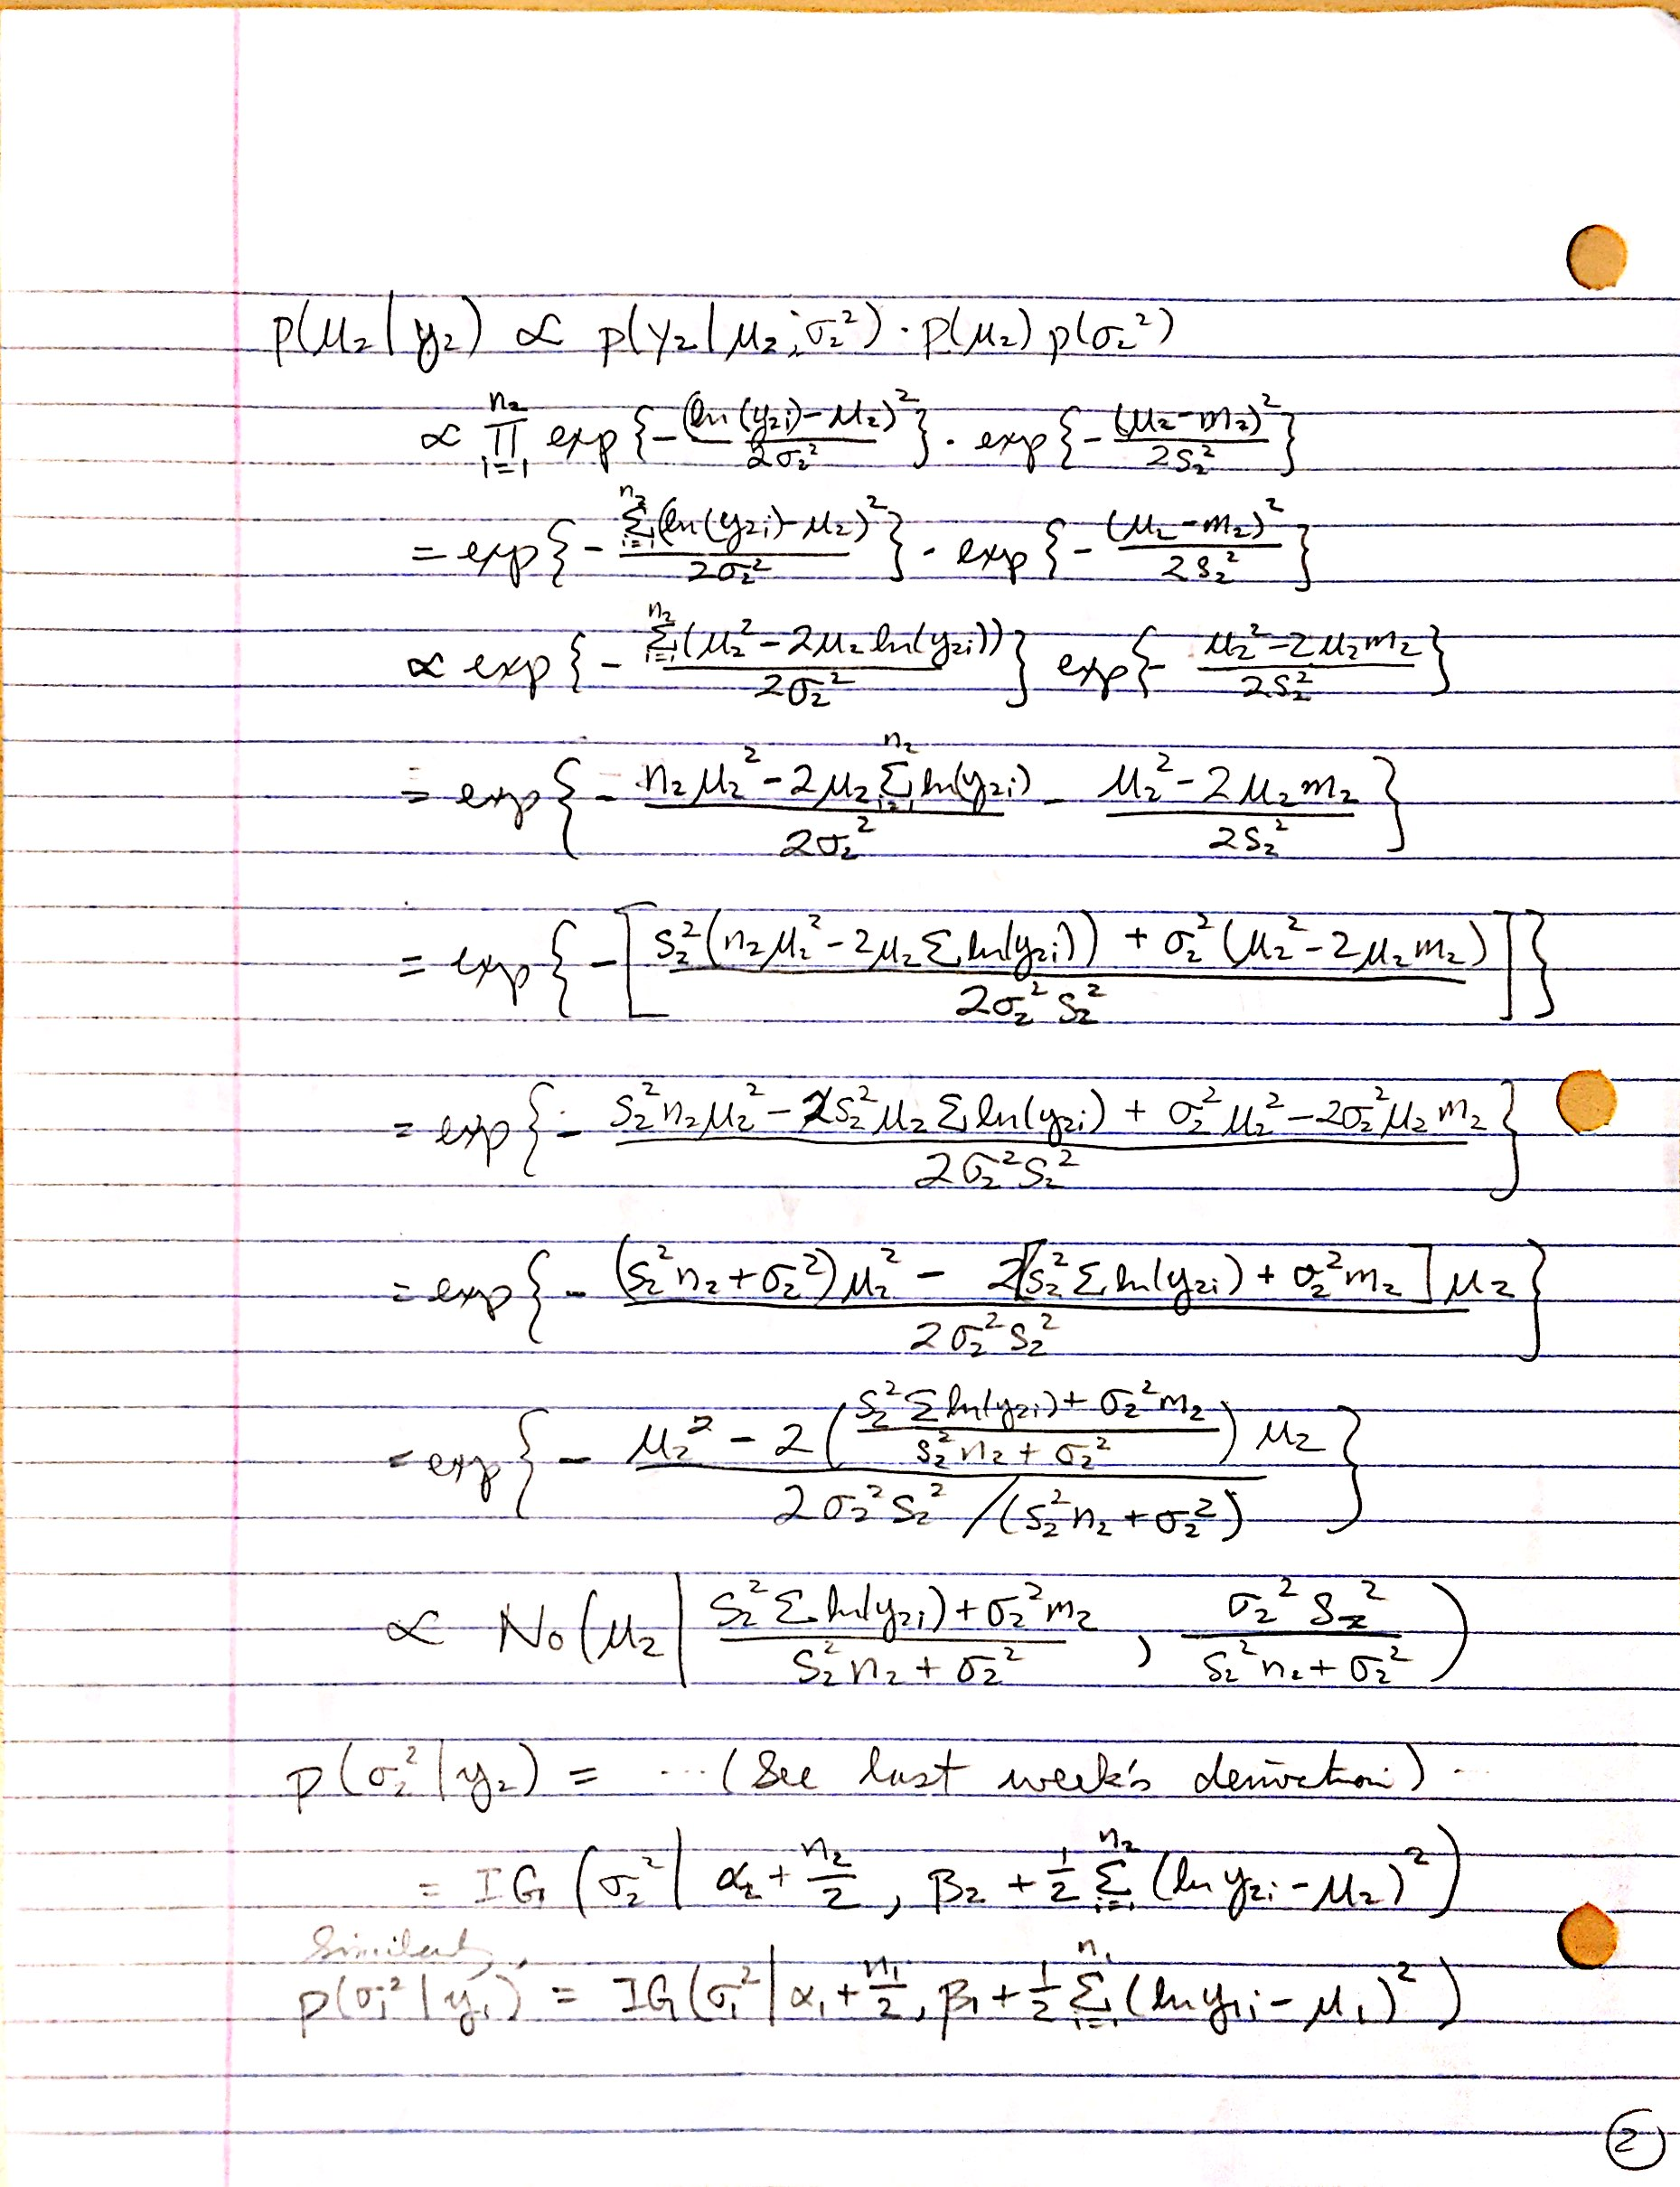
\includegraphics[scale = 0.23]{page2.jpg}\\
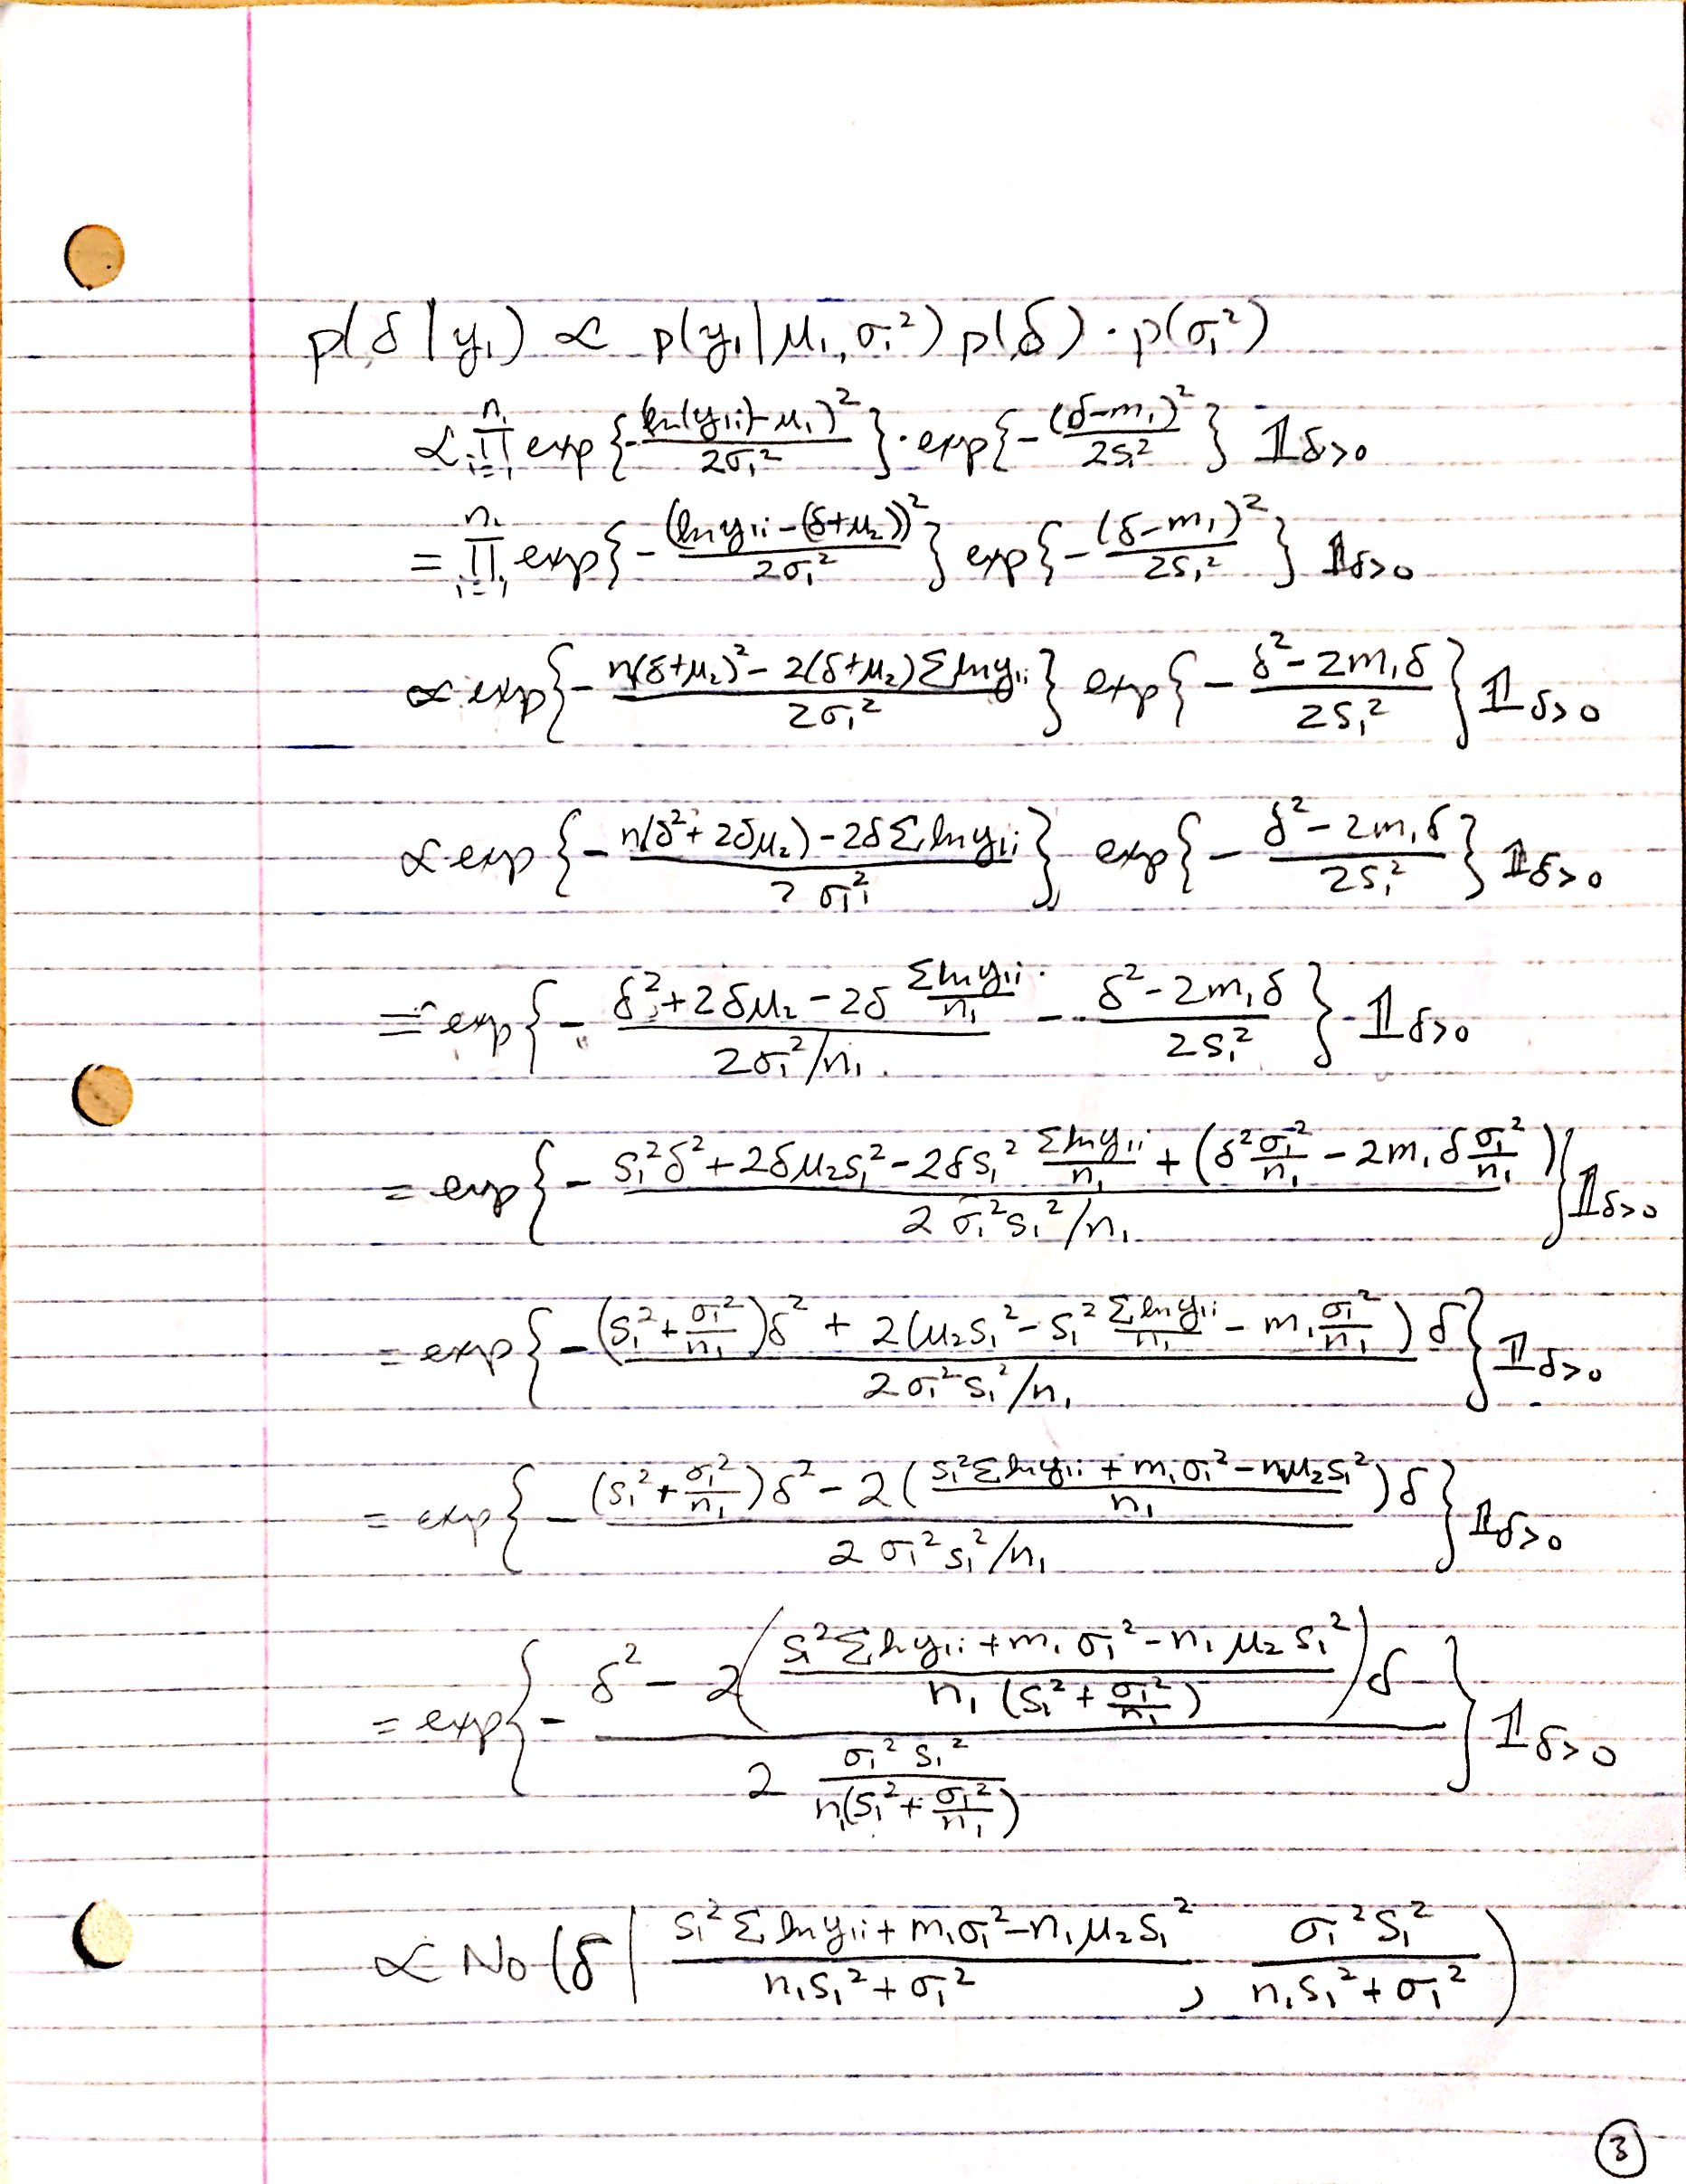
\includegraphics[scale = 0.23]{page3.jpg}\\
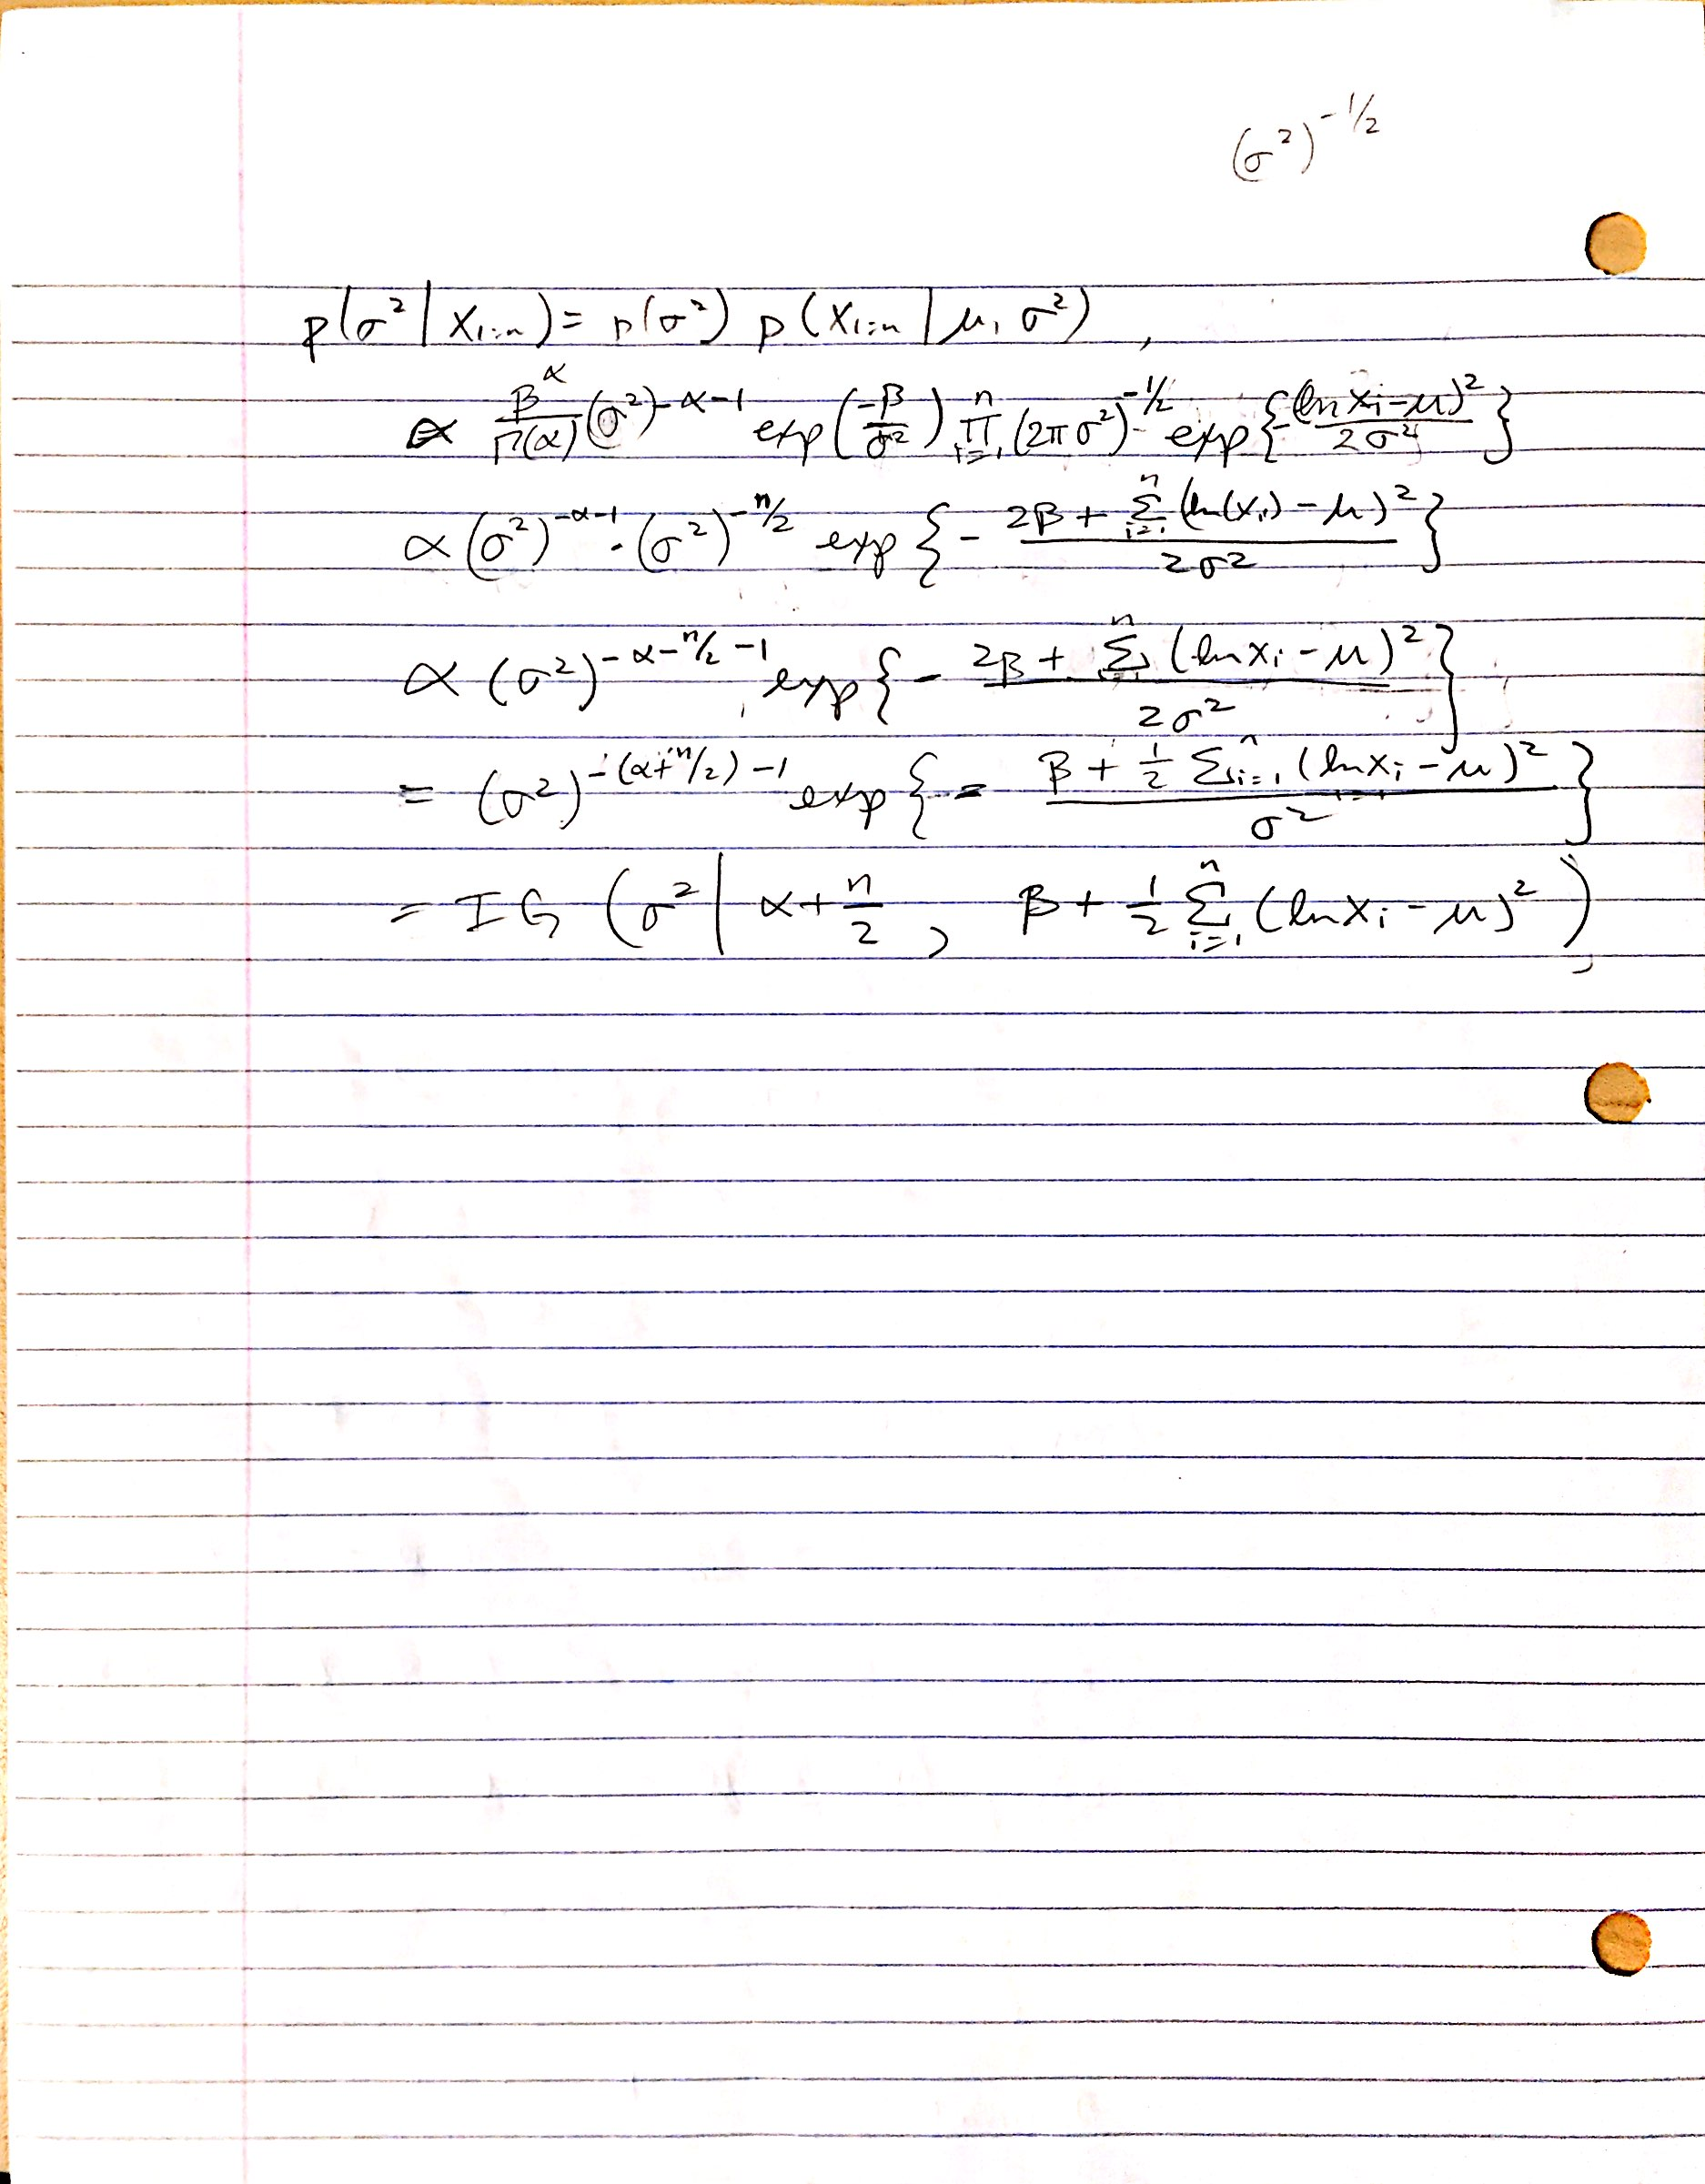
\includegraphics[scale = 0.23]{page4.jpg}\\

\pagebreak
\item The sampler has converged. See traceplots and running averages below:

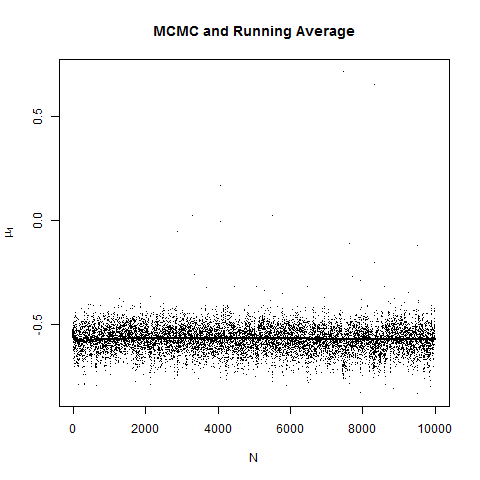
\includegraphics[scale = 0.4]{mu1.png}
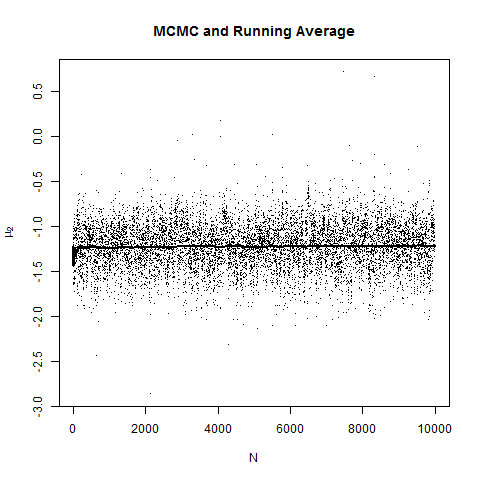
\includegraphics[scale = 0.4]{mu2.png}\\
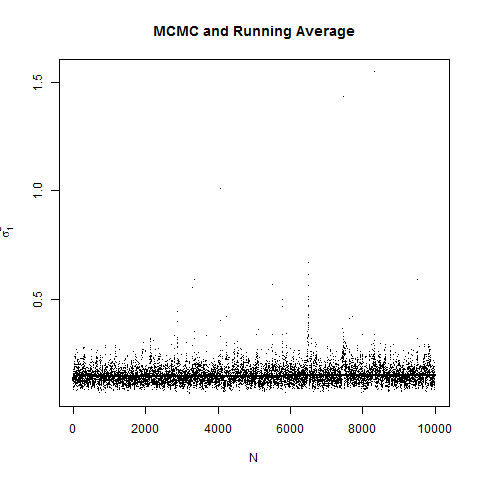
\includegraphics[scale = 0.4]{sig1.png}
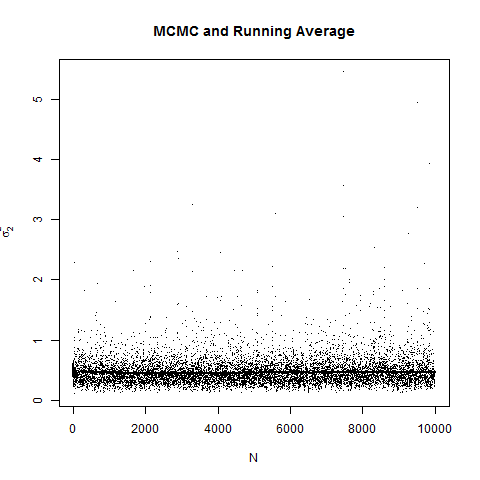
\includegraphics[scale = 0.4]{sig2.png}\\

\pagebreak
\item Below is a plot of $\mu_2$ vs. $\mu_1$:

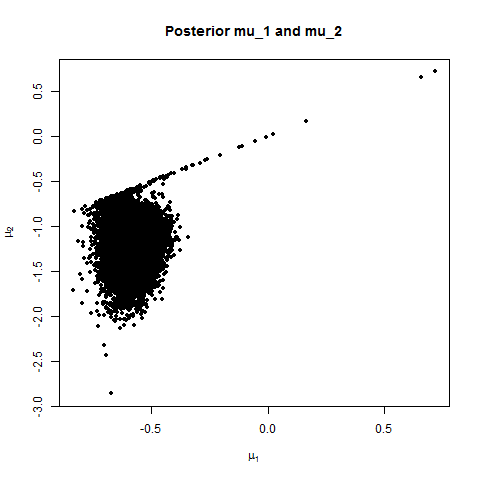
\includegraphics[scale = 0.5]{post.png}

\item 
\begin{itemize}
\item Number of days in the sample which are weekdays: 77.6965. 95\% posterior credible interval is [58, 92].
\item Probability that the technician is coming in less often on weekends than on weekdays: 0.7908.
\end{itemize}

\item Below are point estimates and 95\% confidence intervals:
\begin{center}
\begin{tabular}{r||c|c}
Lab 11 & Mean & Confidence Interval \\ \hline
$\mu_1$ & -0.5728062 & [-0.7031991, -0.4558429] \\ \hline
$\mu_2$ & -1.218221 & [-1.7240026, -0.7504473] \\ \hline
$\sigma_1^2$ & 0.1494581 & [0.09059487, 0.24865874] \\ \hline
$\sigma_2^2$ & 0.46506 & [0.1903877, 1.0277780]
\end{tabular}
\end{center}

Below are point estimates and 95\% confidence intervals from lab 10:

\begin{center}
\begin{tabular}{r||c|c}
Lab 10 & Mean & Confidence Interval \\ \hline
$\mu_1$ & -0.4708718 & [-0.5466545, -0.3949325] \\ \hline
$\mu_2$ & -1.377839 & [-1.5240060, -1.2294750] \\ \hline
$\sigma_1^2$ & 0.1104881 & [0.07978934, 0.15334020] \\ \hline
$\sigma_2^2$ & 0.1597617 & [0.09405123, 0.26961285]
\end{tabular}
\end{center}
In general, the point estimates of parameters are comparable between results from lab 10 and lab 11, but the variance is larger in lab 11. However, the point estimates for $\sigma_2^2$ is very different between the two samplers.
\end{enumerate}
\pagebreak
See below for R code:
\listinginput[1]{1}{lab11.r}

\end{document}